% Gráficos, separados para no generar bardo
\def\doceiA{
  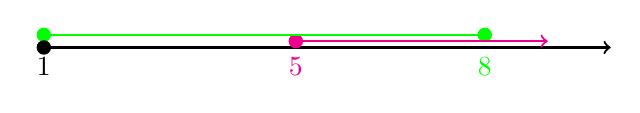
\begin{tikzpicture}[scale=0.8, baseline=0]
    % Number line
    \draw[thick, ->,] (1,0) -- (10,0);
    % Interval
    \draw[fill=magenta, color=magenta] (5,0.1) circle (3pt);
    \draw[fill=green, color=green] (8,0.2) circle (3pt);
    \draw[fill=green, color=green] (1,0.2) circle (3pt);
    \draw[fill=black] (1,0) circle (3pt);
    \draw[-, green, thick] (1,0.2) -- (8,0.2);
    \draw[->, magenta, thick] (5,0.1) -- (9,0.1);
    \node at (1,-0.3) {1};
    \node [color=magenta]at (5,-0.3) {5};
    \node[color=green] at (8,-0.3) {8};
  \end{tikzpicture}
}

\def\doceiiA{
  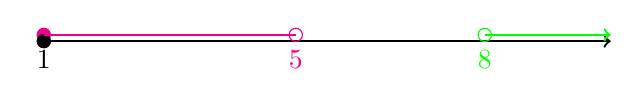
\begin{tikzpicture}[scale=0.8, baseline=0]
    % Number line
    \draw[thick, ->,] (1,0) -- (10,0);
    % Interval
    \draw[color=magenta] (5,0.1) circle (3pt);
    \draw[color=green] (8,0.1) circle (3pt);
    \draw[fill=magenta, color=magenta] (1,0.1) circle (3pt);
    \draw[fill=black] (1,0) circle (3pt);
    \draw[-, magenta, thick] (1,0.1) -- (5,0.1);
    \draw[->, green, thick] (8,0.1) -- (10,0.1);
    \node at (1,-0.3) {1};
    \node [color=magenta]at (5,-0.3) {5};
    \node[color=green] at (8,-0.3) {8};
  \end{tikzpicture}
}

\def\doceiiE{
  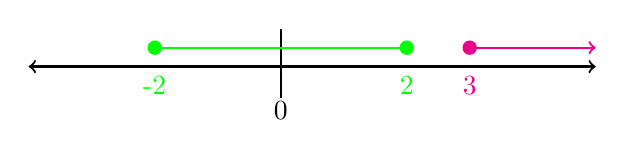
\begin{tikzpicture}[scale=0.8, baseline=0]
    % Number line
    \draw[thick, <->,] (-4,0) -- (5,0);
    \draw[thick] (0,-0.5) -- (0,0.6);
    \node[color=black] at (0,-0.7) {0};
    % Intervals
	% Set A
    \draw[fill=magenta, color=magenta] (3,0.3) circle (3pt);
    \draw[->, magenta, thick] (3,0.3) -- (5,0.3);
    \node[color=magenta] at (3,-0.3) {3};
	%Set B
    \draw[fill=green, color=green] (2,0.3) circle (3pt);
    \draw[fill=green, color=green] (-2,0.3) circle (3pt);
    \draw[-, green, thick] (-2,0.3) -- (2,0.3);
    \node[color=green] at (2,-0.3) {2};
    \node[color=green] at (-2,-0.3) {-2};

  \end{tikzpicture}
}

\def\doceiiicero{
  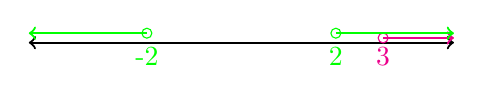
\begin{tikzpicture}[scale=0.6, baseline=0]
    % Number line
    \draw[thick, <->,] (-4.5,0) -- (4.5,0);
    % Interval
    \draw[color=magenta] (3,0.1) circle (3pt);
    \draw[color=green] (2,0.2) circle (3pt);
    \draw[color=green] (-2,0.2) circle (3pt);

    \draw[->, magenta, thick] (3,0.1) -- (4.5,0.1);
    \draw[<-, green, thick] (-4.5,0.2) -- (-2,0.2);
    \draw[->, green, thick] (2,0.2) -- (4.5,0.2);

    \node[color=magenta] at (3,-0.3) {3};
    \node[color=green] at (2,-0.3) {2};
    \node[color=green] at (-2,-0.3) {-2};
  \end{tikzpicture}
}

\def\doceiiiuno{
  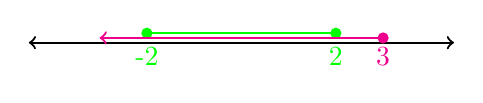
\begin{tikzpicture}[scale=0.6, baseline=0]
    % Number line
    \draw[thick, <->,] (-4.5,0) -- (4.5,0);
    % Interval
    \draw[fill=magenta, color=magenta] (3,0.1) circle (3pt);
    \draw[fill=green, color=green] (2,0.2) circle (3pt);
    \draw[fill=green, color=green] (-2,0.2) circle (3pt);

    \draw[<-, magenta, thick] (-3,0.1) -- (3,0.1);
    \draw[-, green, thick] (-2,0.2) -- (2,0.2);

    \node[color=magenta] at (3,-0.3) {3};
    \node[color=green] at (2,-0.3) {2};
    \node[color=green] at (-2,-0.3) {-2};
  \end{tikzpicture}
}

\def\doceiiidos{
  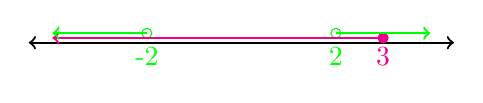
\begin{tikzpicture}[scale=0.6, baseline=0]
    % Number line
    \draw[thick, <->,] (-4.5,0) -- (4.5,0);
    % Interval
    \draw[fill=magenta, color=magenta] (3,0.1) circle (3pt);
    \draw[color=green] (2,0.2) circle (3pt);
    \draw[color=green] (-2,0.2) circle (3pt);

    \draw[<-, magenta, thick] (-4,0.1) -- (3,0.1);
    \draw[<-, green, thick] (-4,0.2) -- (-2,0.2);
    \draw[->, green, thick] (2,0.2) -- (4,0.2);

    \node[color=magenta] at (3,-0.3) {3};
    \node[color=green] at (2,-0.3) {2};
    \node[color=green] at (-2,-0.3) {-2};
  \end{tikzpicture}
}

\def\doceiiitres{
  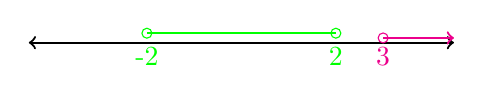
\begin{tikzpicture}[scale=0.6, baseline=0]
    % Number line
    \draw[thick, <->,] (-4.5,0) -- (4.5,0);
    % Interval
    \draw[color=magenta] (3,0.1) circle (3pt);
    \draw[color=green] (2,0.2) circle (3pt);
    \draw[color=green] (-2,0.2) circle (3pt);

    \draw[->, magenta, thick] (3,0.1) -- (4.5,0.1);
    \draw[-, green, thick] (-2,0.2) -- (2,0.2);

    \node[color=magenta] at (3,-0.3) {3};
    \node[color=green] at (2,-0.3) {2};
    \node[color=green] at (-2,-0.3) {-2};
  \end{tikzpicture}
}

% Gráficos, separados para no generar bardo
% =====================================
% =====================================
% =====================================

\begin{enunciado}{\ejercicio}
  \begin{enumerate}[label=\roman*)]
    \item\label{12-itemi}
          Decidir si las siguientes proposiciones son verdaderas o falsas, justificando debidamente:
          \begin{multicols}{2}
            \begin{enumerate}[label=\alph*)]
              \item $\paratodo n \en \naturales,\, n \geq 5 \otext n \leq 8$.
              \item $\existe n \en \naturales \talque n \geq 5 \y n\leq 8.$
              \item $\paratodo n \en \naturales, \existe m \en \naturales \talque m > n$.
              \item $\existe n \en \naturales \talque \paratodo m \en \naturales, m >n$.
              \item\label{12-item1} $\paratodo x \en \reales,\, x > 3 \entonces x^2 > 4$.
              \item\label{12-item2} Si $n$ es un natural terminado en 4, entonces $n$ es par.
              \item Si $z$ es un número real, entonces $z \en \complejos$.
            \end{enumerate}
          \end{multicols}

    \item Negar las proposiciones anteriores, y en cada caso verificar que la proposición negada tiene el valor de verdad
          opuesto al de la original.

    \item Reescribir las proposiciones \ref{12-item1} y \ref{12-item2} del item \ref{12-itemi}
          utilizando las equivalencias del ejercicio \ref{ej:10}\ref{10-1-i}
  \end{enumerate}
\end{enunciado}

\begin{enumerate}[label=\roman*)]
  \item

        \begin{enumerate}[label=\alph*)]
          \item $\paratodo n \en \naturales,\, n \geq 5 \otext n \leq 8$.

                La proposición es verdadera. El conjunto descrito por $\set{ n \en \naturales \talque n \leq 8 \otext n \geq 5} = \naturales$
                \doceiA                        \par
                \red{¿Se puede justificar con un gráfico? \blue{$\to$ ¡Sí!}}

          \item $\existe n \en \naturales \talque n \geq 5 \y n\leq 8.$\par
                La proposición es verdadera, en este caso es cuestión de encontrar solo un valor que cumpla, $n = 6$

          \item $\paratodo n \en \naturales, \existe m \en \naturales \talque m > n$.\par
                La proposición es verdadera, si se elige por ejemplo a $m = n+1$

          \item $\existe n \en \naturales \talque \paratodo m \en \naturales, m >n$.\par
                La proposición es falsa, el único $n \en \naturales$ que no tiene un número menor estricto es el 1. Pero la condición
                dice que $\paratodo m \en \naturales$ se debe cumplir y si m $1 \nless 1$

          \item $\paratodo x \en \reales,\, x > 3 \entonces x^2 > 4$.\par
                La proposición es verdadera. Si $x > 3 \entonces x^2 > 9 \flecha{en}[particular] x^2 > 9 > 4 \entonces x^2 > 4$

          \item $n \en \naturales$, cuyo último dígito es 4. Entonces hay un $m \en \naturales_{\geq 0}$ con su último dígito 0 tal que
                $$
                  n = m + 4.
                $$
                Si un número tiene 0 como último dígito, debe ser múltiplo de 10, es decir
                $m = 10 \cdot m'$ con $m' \en \naturales_{\geq 0} $. Por lo que se puede escribir a $n$ como:
                $$
                  n = \green{10} \cdot m' + \magenta{4} =
                  \green{2 \cdot 5} \cdot m' + \magenta{2 \cdot 2} =
                  2 \cdot (5 m' + 2) =
                  2 \cdot m^{''},
                $$ con $m^{''} \en \naturales_{\geq 2}$.
                $$
                  n = 2m^{''}.
                $$
                Si un natural termina con 4, es par. La proposición es verdadera.

          \item Si $z$ es un número real, entonces $z \en \complejos$.\par
                Están proponiendo que dado
                $z \en \reales \entonces z \en \complejos$.
                Dado que
                $\reales \subseteq \complejos =
                  \set{a \en \reales,\, b\en \reales \talque a + i b}$,
                con $i^2 = -1$
                Por lo tanto para $b = 0$, podría generar todo $\reales$.
        \end{enumerate}

        \separadorCorto

  \item
        \begin{enumerate}[label=\alph*)]
          \item $\existe n \en \naturales,\, n < 5 \y n > 8$.\par
                $A =  \set{n \en \naturales \talque n < 5 \y n > 8} = \vacio \entonces \noexiste n$ que cumpla lo pedido.\par
                \doceiiA \par

          \item $\paratodo n \en \naturales \talque n < 5 \otext n > 8$.

                La proposición es falsa, $n = 6$ no cumple estar en ese conjunto.

          \item $\existe n \en \naturales, \paratodo m \en \naturales \talque m \leq n$.\par
                La proposición es falsa, porque el conjunto $\naturales$ no tiene un máximo. $n = m+1$.

          \item $\paratodo n \en \naturales \talque \existe m \en \naturales, m \leq n$.\par
                La proposición es verdadera, el único $m \en \naturales$ que cumple eso es el $m = 1$.

          \item $\existe x \en \reales,\, x > 3 \land x^2 \leq 4$.\par          		
                La proposición es falsa. El nuevo conjunto propuesto es vacío.\par
                \[
                  \llaves{c}{
                    \magenta{A = \set{x \en \reales \talque x > 3}} 
                    \\
					\ytext
					\\	
                    \green{B = \set{x \en \reales \talque |x| \leq 2}}
                  } \to \doceiiE
                \]

          \item \textit{Si $n$ es un natural que no termina en 4 entonces no es par}.\par
                Un contraejemplo bastaría para probar que esto es falso: El número 12. No termina con el
                número cuatro y es par, ya que $12 = 2\cdot 6$.

          \item Si $z$ no es un número real, entonces $z \notin \complejos$.\par
                La proposición es falsa. Están proponiendo que dado $z \notin \reales \entonces z \notin \complejos$.
                Si $z = i$, se prueba lo contrario.
                Dado que $i \notin \reales$, pero  $i \en \complejos$
        \end{enumerate}

  \item
          e)

        $$
          \begin{array}{|c|c|c|c|}
            \hline
            p \entonces q           & \paratodo x \en \reales, x > 3 \entonces x^2 > 4 & \doceiiicero & A \stacktext{?}{\subseteq} B \Tilde                  \\
            \hline
            \sim q \entonces \sim p & x^2 \leq 4 \entonces x \leq 3                    & \doceiiiuno  & A \stacktext{?}{\subseteq} B \Tilde                  \\
            \hline
            \sim p \lor q           & x \leq 3 \otext x^2 > 4                              & \doceiiidos  & A \union B \igual{?} \universo \Tilde                \\
            \hline
            \sim (p \lor \sim q)    & \sim (x > 3 \y x^2 \leq 4 )                      & \doceiiitres & (A \inter B)^c \igual{?} \vacio^c = \universo \Tilde \\
            \hline
          \end{array}
        $$
\end{enumerate}

% Contribuciones
\begin{aportes}
  %% iconos : \github, \instagram, \tiktok, \linkedin
  %\aporte{url}{nombre icono}
  \item \aporte{\dirRepo}{Nad Garraz \github}
  \item \aporte{https://www.instagram.com/juaanparajo}{Juan Parajó \instagram}
  \item \aporte{https://github.com/APNieto/}{Ale Nieto \github}
\end{aportes}
